%%This is a very basic article template.
%%There is just one section and two subsections.
%\documentclass{sig-alternate}


\documentclass[conference]{IEEEtran}

% \usepackage{graphicx}
% \usepackage{subfig}
% \usepackage{amsmath}
% 
% \begin{document}
% 
%    \conferenceinfo{GECCO'13,} {July 6-10, 2013, Amsterdam, The Netherlands.}
%     \CopyrightYear{2013}
%     \crdata{TBA}
%     \clubpenalty=10000
%     \widowpenalty = 10000
% 
% \title{Robot Coverage Control by Evolved Neuromodulation}
% 
% \numberofauthors{4}
% 
% %\author{Kyle I. Harrington, Emmanuel Awa,\\ Sylvain Cussat-Blanc, Jordan Pollack}
% 
% \author{
% \alignauthor
% Kyle I. Harrington\\
%        \affaddr{DEMO Lab}\\
%        \affaddr{Computer Science}\\
%        \affaddr{Brandeis University}\\
% \email{kyleh@cs.brandeis.edu}
% \alignauthor
% Emmanuel Awa\\
%        \affaddr{DEMO Lab}\\
%        \affaddr{Computer Science}\\
%        \affaddr{Brandeis University}\\
%        \email{eawa@brandeis.edu}
% \and
% \alignauthor
% Sylvain Cussat-Blanc\\
% 	\affaddr{University of Toulouse} \\
% 	\affaddr{21 all\'ee de Brienne}\\
% 	\affaddr{31015 Toulouse, FRANCE}\\
% 	\email{\mbox{sylvain.cussat-blanc@irit.fr}}
% \alignauthor
% Jordan Pollack\\
%        \affaddr{DEMO Lab}\\
%        \affaddr{Computer Science}\\
%        \affaddr{Brandeis University}\\
% 	   \email{pollack@brandeis.edu}
% }

\usepackage{stmaryrd}
%\usepackage[noadjust]{cite}
\usepackage{amsfonts}
% If the IEEEtran.cls has not been installed into the LaTeX system files,
% manually specify the path to it: e.g.,
% \documentclass[conference]{../sty/IEEEtran}

\usepackage{graphicx,times,amsmath,subfig} % Add all your packages here

% correct bad hyphenation here
\hyphenation{op-tical net-works semi-conduc-tor IEEEtran}

\IEEEoverridecommandlockouts    % to create the author's affliation portion
                % using \thanks

\textwidth 178mm    % <------ These are the adjustments we made 10/18/2005
\textheight 239mm   % You may or may not need to adjust these numbes again
\oddsidemargin -7mm
\evensidemargin -7mm
\topmargin -6mm
\columnsep 5mm

\begin{document}


% paper title: Must keep \ \\ \LARGE\bf in it to leave enough margin.
\title{\ \\ \LARGE\bf Robot Coverage Control by Evolved
Neuromodulation\thanks{K. Harrington, E. Awa, and J. Pollack are with the
DEMO Lab, Department of Computer Science, Brandeis University, Waltham, MA, USA.
S. Cussat-Blanc is with the University of Toulouse, Toulouse, France. Corresponding
email: kyleh@cs.brandeis.edu (eawa@brandeis.edu, sylvain.cussat-blanc@irit.fr, pollack@brandeis.edu)}}

\author{Kyle I. Harrington, Emmanuel Awa, Sylvain Cussat-Blanc, Jordan Pollack}

\date{}

\maketitle

\begin{abstract}
An important connection between evolution and learning was made over a century
ago and is now termed as the Baldwin effect. Learning acts as a guide for an
evolutionary search process. In this study reinforcement learning agents are
trained to solve the robot coverage control problem. These agents are improved
by evolving neuromodulatory gene regulatory networks (GRN) that influence the
learning and memory of agents. Agents trained by these neuromodulatory GRNs can
consistently generalize better than agents trained with fixed parameter
settings. This work introduces evolutionary GRN models into the context of
neuromodulation and illustrates some of the benefits that stem from
neuromodulatory GRNs.
\end{abstract}

\section{Introduction}

As biological organisms have evolved, there has been a general trend that
appears to favor the selection of individuals with plasticity via learning.
While basic hard-coded behaviors can be quite powerful and may even be complex,
such behaviors do not often translate between environmental contexts.
Furthermore, there is evidence from studies of the interaction between evolution
and learning that, in tandem, both processes can exhibit a synergistic
expediting effect \cite{hinton1987learning, Ancel2000}. This has been termed the
Baldwin expediting effect \cite{Baldwin1896}, which states that plasticity (learning) can
facilitate genotype improvement by providing gradient information. We extend
this research by evolving an artificial gene regulatory network (GRN), which
dynamically modulates agent learning. In this study the neuromodulatory GRN
allows agents to dynamically regulate learning and memory according to what the
agent senses in its environment.

The interaction between evolution and learning has a long-standing history
\cite{hinton1987learning}. In their pioneering work, Hinton and Nowlan
simultaneously evolve static and learnable neural network weights. They find
that the ability to learn improves the evolvability of the networks. This
improvement is expected to be primarily caused by the gradient information that
learning provides about how far a network is from the correct solution.
Since this initial finding there have been a number of studies which explore the
Baldwin expediting effect \cite{Wagner1996, Ancel2000, Ancel2000a}, where a
general consensus finds that the problem domain can have a significant impact on
how much improvement, or even detriment, plasticity provides.

GRNs are a fundamental and pervasive structure in biology. Many motile bacterial
cells use GRNs to modulate their flagellate motor allowing for chemotaxis,
phototaxis, and other environment seeking behaviors. This property has been
exploited for the control of robots with artificial GRNs \cite{Ziegler:2001:AL,
Nicolau:2010:EuroGP, Joachimczak10, CussatBlanc2012b}, where robots evolved
useful navigation behaviors. Other research has extended the application of
artificial GRNs to other robot control problems.

Artificial neural networks are one of the most used models of
biologically-plausible learning because of their relation to biological neural
networks. While the field of neural networks itself has had a tumultuous
history, researchers continued to pursue studies of hierarchical learning
structures, such as the Hinton and Nowlan's layering of generational evolution
and lifetime learning. During the first neural network rennaisance a method
for learning with cascading neural networks was proposed \cite{Pollack1986}. In
a two-network cascade one network acts as a function network while the other
network defines context by specifying the weights of the function network. In
this work we consider an internal cascading mechanism, whereby a gene regulatory
network produces neuromodulators that alter learning and memory.

Ackley and Littman designed a system to test learning and evolution with a
modified backpropagation network in an artificial life context \cite{Ackley1991}. In
their study agents evolve the initial weights of learnable-control neural
networks and fixed reward-estimation networks. Fixed reward-estimation networks
are used to produce a reinforcement signal for an adapted version of the
backpropagation learning algorithm. The complexity of their environment and
relatively open-ended task require such an estimated reinforcement signal.
However, the robot coverage control problem which we address (explained in the
following section) has a clear objective with a minimal natural framing in the
context of reinforcement learning. This reduces the number
of factors that may obscure analysis of the resultant behaviors.

We begin this paper with an overview of the robot coverage control problem.
We then explain the reinforcement learning algorithm which is used for robot
control. The gene regulatory networks that are used for neuromodulation are then
introduced. Finally, we present the specific instantiation of the problem and
the algorithms used in our experiments, and the experiments themselves. We then
conclude with a discussion of the benefits of evolving neuromodulatory
gene regulatory networks that influence learning and memory.

\section{Coverage Control}

\begin{figure}
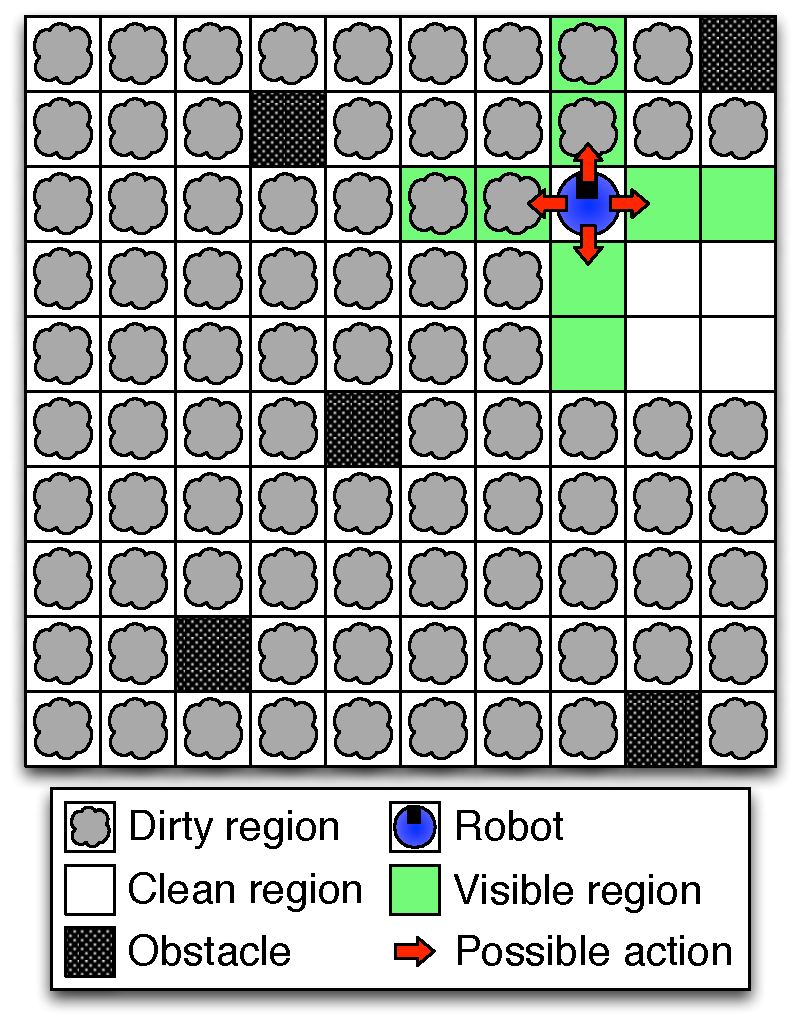
\includegraphics[width=\linewidth]{img/environment.pdf}
\caption{The environment for the CCP problem.}
\label{fig:environment}
\end{figure}

Some of the classic examplar problems of artificial intelligence involve the
control of agents in 2D worlds \cite{Russell1995}. A high-impact
problem in this domain is the control of robotic vacuum cleaners. The general
robotic cleaner market is currently approaching the billion dollar mark. A robot
vacuum cleaner is an agent that must avoid potentially mobile obstacles and
clean ephemerally accumulating dirt within some region. Other tasks, such as
charging are ignored in this study. The objective of the robot is to clean all
the dirt that has accumulated. In spite of limited sensors and the inability to
maintain a sufficiently accurate internal map, this challenge of the task is to
uniformly covering the region.

% The problem of uniformly covering a region is related to the traveling
% salesperson problem (TSP). The TSP is a NP-hard problem where the salesperson
% attempts to find the shortest path that visits every customer exactly once.
% Instances of the TSP are represented as sets of nodes, and solutions are edges
% through the nodes. The coverage control problem (CCP) is to find the shortest
% path that visits every node at least once. Instances of the CCP are still
% represented as nodes; however, solutions are form multigraphs with multiple
% edges existing between nodes.

Robot coverage problems have a long standing history in evolutionary
computation. One of the first genetic programming (GP) studies was on what has
come to be called the ``lawnmower'' problem \cite{dickmanns1987genetische}. The
lawnmower problem is an instance of the control coverage problem (CCP) in a uniform environment, often with
turn-based navigation and the ability to jump. The use of modular structures have
been shown to facilitate solving the lawnmower problem in GP
\cite{koza1994genetic}. The lawnmower problem, and other versions of the CCP,
have been extensively studied in the field of GP, but a review of GP techniques
is beyond the scope of this paper. However, we highlight an observation that
was revealed for a version of the CCP with obstacles \cite{SpectorGPTPTags}. In
this study the meanings of evolved behavioral modules were investigated, and it
was found that optimal solutions contained modules that encoded short action sequences
which were then iterated to solve the CCP. This observation suggests that 
successful agents may only need to learn a few short, but useful, action sequences. 
An example illustration of the CCP is shown in Figure \ref{fig:environment}. 

The CCP has also been studied from a multi-robot perspective. In \cite{Morlok2007},
simple hard-coded heuristics, such as wall-seeking behavior, are used by
multiple robots to solve the CCP in a distributed manner. Optimal control for
multi-robot coverage problems in mobile sensing networks has been explored
analytically \cite{Cortes2004}. An overview of distributed algorithms for 
the CCP can be found in \cite{Choset2001}.

\section{Reinforcement Learning}

Reinforcement learning is a reward-based learning algorithm that allows agents
to learn from experience. More formally, reinforcement
learning (RL) is a mathematical framework for learning from a reward signal that
is derived from Bellman's equation for optimal control \cite{Sutton1998}. One of
the most important forms of RL is temporal-difference (TD) RL. TD-RL is a method
for learning optimal behavior from changes in state and reinforcement by error
prediction \cite{Sutton1988}. TD-RL agents learn an expected return that will be
received after taking an action in any state. Strong correlations with this type of
error predictive behavior have been found in studies of dopamine neurons
\cite{Schultz1993}. This line of research has continued and is now been
supported by fMRI data of reward processing for tastes, money, and love
\cite{Haber2009}.

TD-RL is used to solve Markov decision processes, which are an extension of
Markov chains to problems framed in terms of state, action, and reward.
Reward signals (such as reinforcement of dirt cleanup) are geometrically encoded
in a table which associates action preferences with states. The basic
TD($\gamma$) algorithm updates one state-action association at a time which
prohibits sequence learning. Eligibility traces are used to associate reward
with sequences of actions by reinforcing a weighted history of most recent
actions. In this study the online version of TD-RL, SARSA (short for,
state-action-reward-state-action), is used. A review of the nuances of
reinforcement learning can be found in \cite{Sutton1998}.

We include a few of the key equations from the RL algorithm which are employed. If we are in state,
$s_t$ at time $t$, then we will take some action $a_t$ which will bring us a
reward $r_t$. This action will also cause us to transition to a new state,
$s_{t+1}$. The SARSA algorithm learns a Q-function, which maps a value to each 
state-action pair, $(s_t,a_t)$. From each state multiple actions, $A_t$, may be taken
which may be a function of $s_t$ (for example, an obstacle may prevent an action
in a given state). Given an optimal Q-function the best action to take is
\begin{equation} argmin_{a_t \in A_t} Q(s_t,a_t).
\end{equation}
\noindent The Q-function is approximated by SARSA with the following update rule
\begin{eqnarray} 
& Q(s_t,a_t) \leftarrow Q(s_t,a_t)+ \nonumber \\ 
& \alpha \big[r_{t+1}+\gamma Q(s_{t+1},a_{t+1}) - Q(s_t,a_t)\big] 
\end{eqnarray}
\noindent where $\alpha$ is the learning rate, and $\gamma$ is the discounting
factor. Given only this update rule it can be difficult to compute the Q-value
for state-action pairs which indirectly contribute to obtaining a reward. This
update method propagates information only to the preceeding state-action pair,
for those that are very distant from the reward, such as in the case of maze
solving problems, this can require a large number of repeated trials. However,
this problem of reward propagation can be partially aleviated by the use of
eligibility traces. Eligibility traces store an accumulating trace of
state-action pairs. The ``memory'' of these state-action pairs can be tuned with
the trace decay parameter $\lambda$. Eligibility traces are updated with
\begin{equation}
e_t(s,a) = 	\begin{cases}
			\gamma \lambda e_{t-1}(s,a) & \mbox{if } s \neq s_t \\ 
			\gamma \lambda e_{t-1}(s,a)+1 & \mbox{if }s = s_t \\
			\end{cases}
\end{equation} 
\noindent By combining the error predictive capabilities of TD-RL with the
state-action sequence memory of eligibility traces we can amplify the effects
of our reward and speed up the learning process. When performing on-policy
learning it is important to ensure that a sufficient amount of exploration
occurs. To this end the $\epsilon$-greedy method is used, where a random
action is taken with $p(\epsilon)$, otherwise the agent's most preferred 
action is taken. However, the RL algorithm can still fail to capitalize on rarely
experienced rewards. 

% SCB: Adding a small transition between RL and NM
In this work, we propose to reduce the effect of rarely experienced rewards by
dynamically modifying the RL parameters according to the local vision of the
robot. With this aim in mind, we propose to use a gene regulatory network to
supervise the adaptation of the coefficient. The end of this section presents
the neuromodulation concept and the GRN model that we used as a neuromodulator.

% The RL framework has been extended to include a number of higher-level features,
% such as learned options (atomic sequences of actions), that have been used to
% improve robot control with a complete map of the environment [Citation]. RL
% can also be used in more complex situations. [Easy to add more here]

%\section{GRN-based Neuromodulation}

% SCB: neuromodulation first and GRN after
%
\section{Neuromodulation}

Neuromodulators are neuropeptides or small molecules, like dopamine and
serotonin. The production of these substances within the cell is controlled by
gene regulatory networks. Neuromodulators change the behavior of neural networks
within individual neurons, amongst neighboring neurons, or throughout the entire
network. Neuromodulation has been found to be pervasive throughout the brain,
and can have drastic consequences on the behavior of neurons and neuronal
circuits \cite{Destexhe2004,Marder2012,Marder2002}. A particularly applicable
example in the realm of robotics is the neuromodulation of motor signals
produced by central pattern generators in the brain and spinal cord
\cite{Katz1995}. It has been found that neuromodulators tune and synchronize
neuromuscular signals \cite{Zhurov2006}.

%We can relate these to foraging tasks with neuromodulation \cite{Montague1995}

We have already noted that the temporal difference learning algorithm for error
prediction has been observed in neural substrates \cite{Schultz1993}.
Dopamine neurons of the ventral tegmental area (VTA) and substantia nigra
exhibit this error predictive behavior. The dopamine system is itself a 
neuromodulatory system. While the temporal difference learning algorithm
extends ideas of reward processing to engineering, there are models of
the dopamine system with closer ties to biology \cite{Montague1996}. These
models also confirm the error predictive behavior found in the brain for a
variety of physiological data including reaction-time and spatial-choice
tasks. Dopamine is an important neuromodulator, especially in learning, but
it is but one of many neuromodulatory substances found in the brain. An
extensive review of computational models of neuromodulation can be found in
\cite{Fellous1998}, and some recent models are reviewed in \cite{Marder2012}.
In this study we focus on the relationship between evolved neuromodulator-producing
GRNs and learned behaviors. 

Computational studies of neuromodulation and neuroendocrine systems are 
becoming a popular method for acheiving dynamic control and learning. A
number of these studies focus on neuromodulatory subsystems with projections
that have diffuse action on the synapses of more classical neurons
\cite{Sporns2002,Risi2009,Soltoggio2008,Pitonakova2013}. On the other hand, this
study develops a model of a single neuron (or homogenous nuclei) with dynamic
regulation of learning and memory by an internal gene regulatory network. The
idea of relating neuromodulatory substances to properties and learning
parameters has been explored \cite{Doya2002,Krichmar2008}, but to the best of
our knowledge has not previously been evolved. As opposed to focusing on
the spatial distribution of neuromodulatory action, our study focuses on
how neuromodulation can be evolved to act in different ways on a learning system.
In a related study, Benuskova and Kasabov evolve GRNs to tune the behavior of a
biologically comprehensive spiking neural network \cite{Benuskova2008}.
In this study, we employ an abstract computational model of a gene regulatory
network to modulate the parameters of a RL agent.

% SCB: GRN goes here
\subsection{Gene regulatory network}

% Artificial GRNs are a biologically-inspired model of the dynamics of a network
% of interacting genes. These models have been applied to biological processes
% such as embryogenesis and agent control. In this study we focus on GRNs for
% agent control, the reader that is interested in GRN-controlled embryogenesis
% is directed to [Citations].

%Formally, artificial GRNs are fully-connected single-layer recurrent neural
%networks with evolvable encodings. 

Our model uses an optimized network of abstract proteins. The inputs of the
agent are translated to protein concentrations that feed the GRN. Output
proteins regulate the reinforcement learning parameters previously described.
This kind of controller has been used in many developmental models of the
literature \cite{Joachimczak08, Doursat09, CussatBlanc2012a} and to control
virtual and real robots \cite{Ziegler:2001:AL, Nicolau:2010:EuroGP,
Joachimczak10, CussatBlanc2012b}.

We have based our regulatory network on Banzhaf's model
\cite{banzhaf:2003:GPTP}. It is designed to be as close as possible to a real
gene regulatory network but neither to be evolved nor to control any kind of
agent. However, Nicolau used an evolution strategy to evolve the GRN to control
a pole-balancing cart \cite{Nicolau:2010:EuroGP}. Though this experiment behaved
consistently, the evolution of the GRN has been an issue. We have decided to
modify the encoding of the regulatory network and its dynamics. In our model, a
gene regulatory network is defined as a set of proteins. Each protein has the
following properties:

\begin{itemize}

\item The protein \emph{tag} coded as an integer between 0 and $p$. The
	upper value $p$ of the domain can be changed in order to control the
	precision of the GRN. In Banzhaf's work, $p$ is equivalent to the size
of a site, 16 bits. 
% We have reduced the precision to 16 because the
% precision of the output values are not a particular requirement in that
% particular application.

\item The \emph{enhancer tag} coded as an integer between 0 and $p$. The
	enhancer tag is used to calculate the enhancing matching factor
	between two proteins.

\item The \emph{inhibitor tag} coded as an integer between 0 and $p$. The
	inhibitor tag is used to calculate the inhibiting matching factor
	between two proteins.

\item The \emph{type} determines if the protein is an \emph{input} protein, the
	concentration of which is given by the environment of the GRN and which
	regulates other proteins but is not regulated, an \emph{output} protein,
	the concentration of which is used as output of the network and which is
	regulated but does not regulate other proteins, or a \emph{regulatory}
	protein, an internal protein that regulates and is regulated by other
	proteins.

\end{itemize}

The dynamics of the GRN is calculated as follow. First, the affinity of a
protein $a$ with another protein $b$ is given by the enhancing factor
$u^{+}_{ab}$ and the inhibiting $u^{-}_{ab}$:
\begin{equation}
u^{+}_{ab}=p-|enh_a-id_b|~~;~~u^{-}_{ab}=p-|inh_a-id_b|
\end{equation}
where $id_x$ is the tag, $enh_x$ is the enhancer tag and $inh_x$
is the inhibiting tag of protein $x$.

The GRN's dynamics are calculated by comparing the proteins two by two using the
enhancing and the inhibiting matching factors. For each protein in the network,
the global enhancing value is given by the following equation:
\begin{equation}
g_i=\frac{1}{N}\sum_j^N{c_je^{\beta u^{+}_{ij}-u_{max}^{+}}}~~;~~h_i=\frac{1}{N}\sum_j^N{c_je^{\beta u^{-}_{ij}-u_{max}^{-}}}
\end{equation}
where $g_i$ (or $h_i$) is the enhancing (or inhibiting) value for a
protein $i$, $N$ is the number of proteins in the network, $c_j$ is the
concentration of protein $j$ and $u_{max}^{+}$ (or $u_{max}^{-}$) is the
maximum enhancing (or inhibiting) matching factor observed. $\beta$ is a
control parameter described hereafter.

The final modification of protein $i$ concentration is given by the following
differential equation:
\begin{equation}
\frac{dc_i}{dt}=\frac{\delta(g_i-h_i)}{\Phi}
\end{equation}
where $\Phi$ is a function that keeps the sum of all protein concentrations
equal to 1.

$\beta$ and $\delta$ are two constants that set up the speed of reaction of the
regulatory network. In other words, they modify the dynamics of the network. $\beta$
affects the importance of the matching factor and $\delta$ affects the level of
production of the protein in the differential equation. The lower both values,
the smoother the regulation. Similarly, the higher the values, the more sudden
the regulation. 



\subsection{GRN-controlled neuromodulation}
 % SCB: this paragraph is already in the experiment part. I have extended the experiment one. 
%Whereas the input proteins of a GRN correspond to the current state of the
%environment, the output proteins act as neuromodulators on the RL parameters. The inputs
%of the GRN correspond to the quantity of dirt in the agent's von Neumann neighborhood,
%the number of unavailable positions in that same neighborhood and the
%reinforcement learning reward. The output of the GRN regulates the reinforcement
%learning by modifying three of its parameters: its learning rate $\alpha$,
%discounting factor $\gamma$ and trace decay parameter $\lambda$.
%The GRN is run for 5 steps before the action is chosen. These 5 steps are
%necessary to reach a stable state of the GRN.

Neuromodulation is incorporated into RL-controlled robots according to the model
shown in Figure \ref{fig:model}.
% SCB: modify the GRN init
When evaluating the performance of a GRN, a robot is initialized with a uniform
Q-function and the GRN is first run with no inputs for 50 steps. The aim of this
initialization is to reach a stable point before exploiting the GRN with inputs.
This phase is necessary because GRNs are known to oscillate chaotically in their
very first steps.

After initialization, the robot is controlled according to the typical SARSA on-line policy learning mechanism;
however, while the agent chooses an action, the proteins of the GRN react and
tune the concentration of the neuromodulators. These neuromodulators are used
for the learning and memory parameters, which are explained in sections III and VI. After
observing the reward from taking an action in the current state, the SARSA
update is applied as usual but with parameters determined by the GRN.

To regulate the RL parameters, the GRN uses the current state of the environment
as inputs. In the CCP problem addressed in this paper, inputs correspond to the
quantity of dirt in the agent's von Neumann neighborhood, the number of
obstructed positions in the same neighborhood, and the current reward (or lack
thereof). The GRN is then run for 5 steps with these inputs before the
learning and memory parameters are used within the RL module. These 5 steps are
necessary to reach a new stable state of the GRN with the new inputs.
%/SCB

\section{Experiment}

In this study we show that the performance of RL-controlled robots on the
CCP is exceeded by RL-controlled robots with neuromodulatory GRNs. The CCP
has a natural framing of reward, which is the dirt that it cleans. The state of
a robot is defined in terms of the robot's perceived surroundings.
In this way, states are not unique with respect to the environment; many
environments will be perceived as the same state. At each timestep the robot can
choose between 4 actions of movement along the von Neumann neighborhood (North,
East, South, West), and the world wraps as a torus. A robot receives a reward of $1$ for moving to a dirty
location, and otherwise receives no reward. These formulations of state, action,
and reward are sufficient to allow RL to control the robot. A diagram of the
experimental environment can be seen in Figure \ref{fig:environment}.

\begin{figure}
%SCB: reducing image
\center
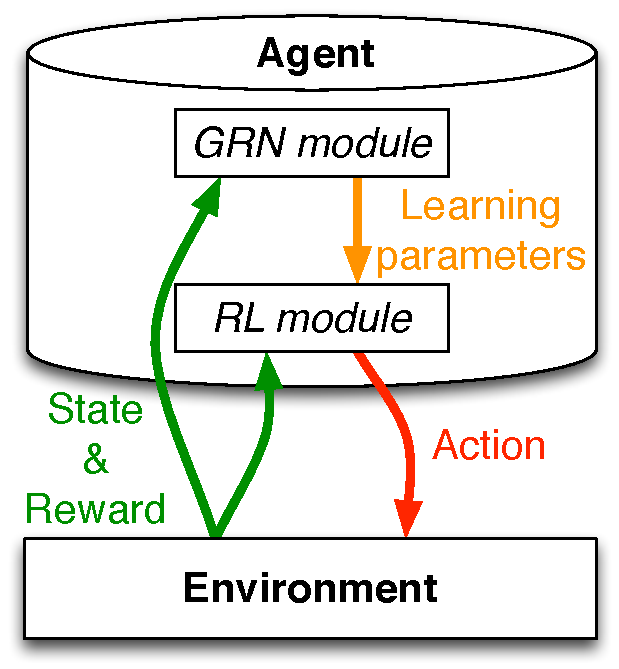
\includegraphics[width=0.75\linewidth]{img/model.pdf}
\caption{A diagram of the model of neuromodulatory control of RL agents.}
\label{fig:model}
\end{figure}

% SCB: in the new GRN-controlled NM
%Neuromodulation is incorporated into RL-controlled robots according to the model
%shown in Figure \ref{fig:model}. 
%%SCB: modify the GRN init
%When evaluating the performance of a GRN,
%a robot is initialized with a uniform Q-function and the GRN is first run for
%50 steps. During this initialization, no inputs are providen to the GRN. The aim is to reach a stable point before exploiting the GRN with inputs. This phase is necessary because the GRN are known to oscillate chaotically in their very first steps. After initialization the robot is 
%controlled according to the typical SARSA on-line policy learning mechanism;
%however, while the agent chooses an action the proteins of the GRN react and
%tune the concentration of the neuromodulators. These neuromodulators are used
%for the learning and memory parameters, $\alpha$, $\gamma$, and $\lambda$. After
%observing the reward from taking an action in the current state, the SARSA
%update is applied as usual but with the parameters that determined by the GRN.

The primary complexity of the environments in our experiments stems from
obstacles, which we expect only requires the learning of short sequences of
actions. Vision extends for a radius of 2 in a cross about the von Neumann
neighborhood. Each location in the discrete 10x10 training grid is represented
with a ternary variable encoding: clean, dirty, or obstructed. The GRN perceives
the environment through three signals: the current reward, fraction of visual field
that is dirty, and the fraction of the visual field that is obstructed. Output
proteins of the GRNs are used to specify the $\alpha$, $\gamma$, and $\lambda$
learning and memory parameters of the reinforcement learning algorithm, as well as
a threshold protein used to normalize the previously mentioned outputs. This
integration of a neuromodulatory GRN and reinforcement learning algorithm is
biologically plausible as well. In this way the GRN acts as a teacher for the
robot, by guiding memory formation, and retention. Parameters are
shown in Table \ref{tbl:parameters}.

The evolutionary algorithm used to evolve the GRNs is similar to a
($\mu$+$\lambda$)-evolution strategy, where subsequent generations are selected
from both a population of parents and children. An initial population of
randomly generated GRNs is created and evaluated. Half of the initial population
is initialized with GRNs which have been filtered to ensure some stability in
their output proteins.
Stable networks pass 2 of 3 criteria which are applied to the parameter values
produced by the network. Each critereon tests that the standard deviation of a
given parameter has a standard deviation less than 0.25 with a mean centered at
0.75 for $\alpha$, $\gamma$ and 0.25 for $\lambda$.
Populations are iteratively updated by creating a candidate child program for
each parent, via mutation or crossover. The child is then evaluated and compared
to its parent. If the child has a lower error than its parent, then it replaces
its parent. The fitness used for evolution is the integral of error over all
training episodes.

Generalization is tested by constructing a set of hypothetical test scenarios
for 6 classes. These scenarios are states that the robot might otherwise
encounter during training, but are only used to test the robot's behavior in a
single state. By only considering a single state-action transition, it becomes
tractable to derandomize the Markovian process and thus consider all possible
outcomes. For a scenario state, $s_{c1}$, the agent may take any action $a_{c1}
\in A_{c1}$. The generalization score is then
\begin{equation}
score_g = ( 1 - 3/4 \epsilon )r(s_{c1},\hat{a}_{c1}) + \epsilon / 4 \displaystyle\sum_{a \in \hat{A}_{c1}} r(s_{c1},a)
\end{equation}
\noindent where $\hat{a}$ is the agent's preferred action and $\hat{A}_{c1}$ is
all actions excluding $\hat{a}$. 5 of the 6 scenario classes correspond to 0-4
dirty squares surrounding the robot, and the 6th class is random. Scenarios are
generated to contain typical distributions of dirt and obstacles encountered
over the course of a training episode. The inclusion of these generalization
scenarios allow the robot to be tested on its response to a wide range of
environmental conditions that may not appear during a training episode.

\begin{table}
\centering
\begin{tabular}{|r|r|}
\hline
Parameter & Value \\
\hline
Sensor radius & 2 \\
World dimensions & 10 x 10 \\
$\epsilon$, p(random move) & 0.1 \\
Training episodes & 50 \\
Steps per episode & 200 \\
Generalization cases & 600 (6 classes) \\
\hline
Input proteins & 3 \\
Output proteins & 4 \\
GRN steps per action & 5 \\
Population size & 50 \\
Max. generations & 50 \\
Tournament size & 7 \\
Number of runs & 25 \\ 
\hline
\end{tabular}
\caption{Parameters used in experiments.}
\label{tbl:parameters}
\end{table}

\section{Analysis of Parameters}

In this analysis we investigate the core parameters of the temporal difference
learning algorithm on the CCP problem for 0 obstacles or various maps with 30
obstacles. The main question we would like to answer is, how do the RL parameters
affect the performance of learning agents on the CCP? In order to do this we 
perform a uniform sampling of the three parameters: $\alpha$, $\gamma$, and
$\lambda$ from $[0.1, 1]$ with an interval of $0.1$. The result of this sampling
is a 4D space where the 3 parameter coordinates are matched with the fitness
achieved by RL agents with these parameters. Agents are trained for 50 training
episodes, where the environment is repopulated with dirt at the end of each
episode. In order to display the parameter maps in a readable fashion we find
the best parameter set from all sampling runs and focus on modal parameter
values. While the subject parameters have highly non-linear effects on the
behavior of RL agents, we articulate some of the general properties they can
have.

\begin{figure}
\centering
\vspace{-5pt}
\subfloat[0 obstacles, $\alpha = 0.1$]{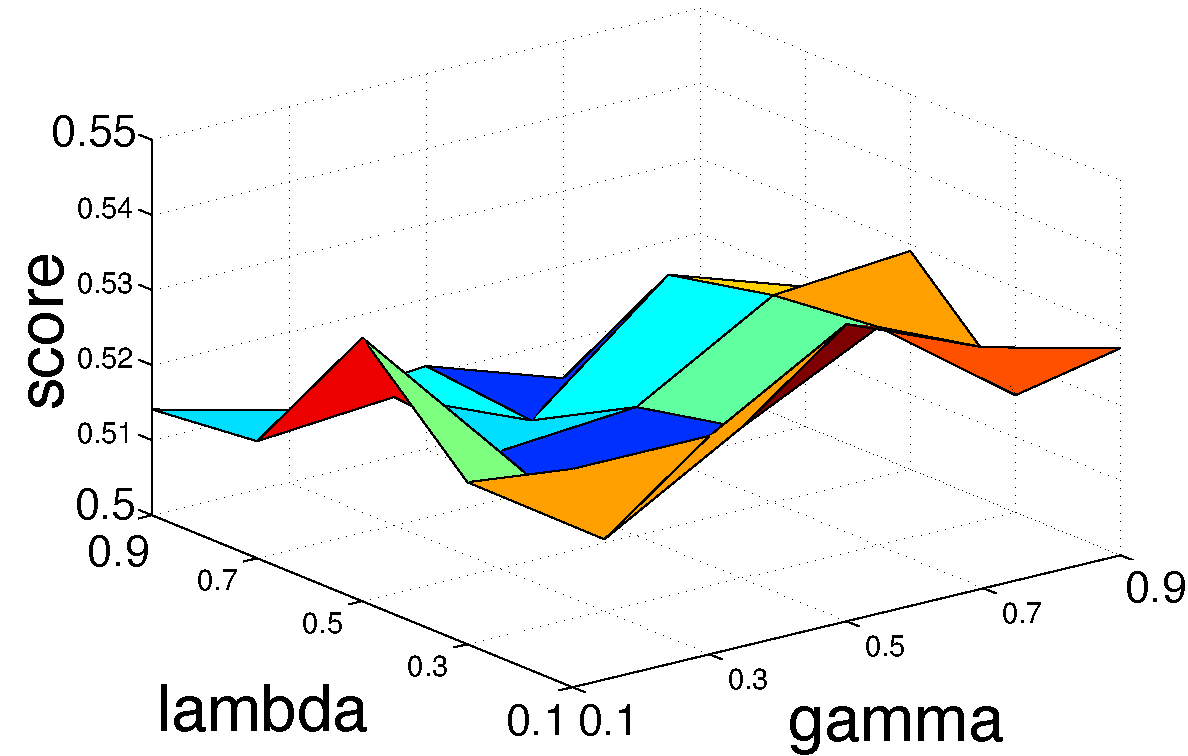
\includegraphics[width=0.5\linewidth]{img/alpha_analysis_0.pdf}}
\subfloat[30 obstacles, $\alpha = 0.7$]{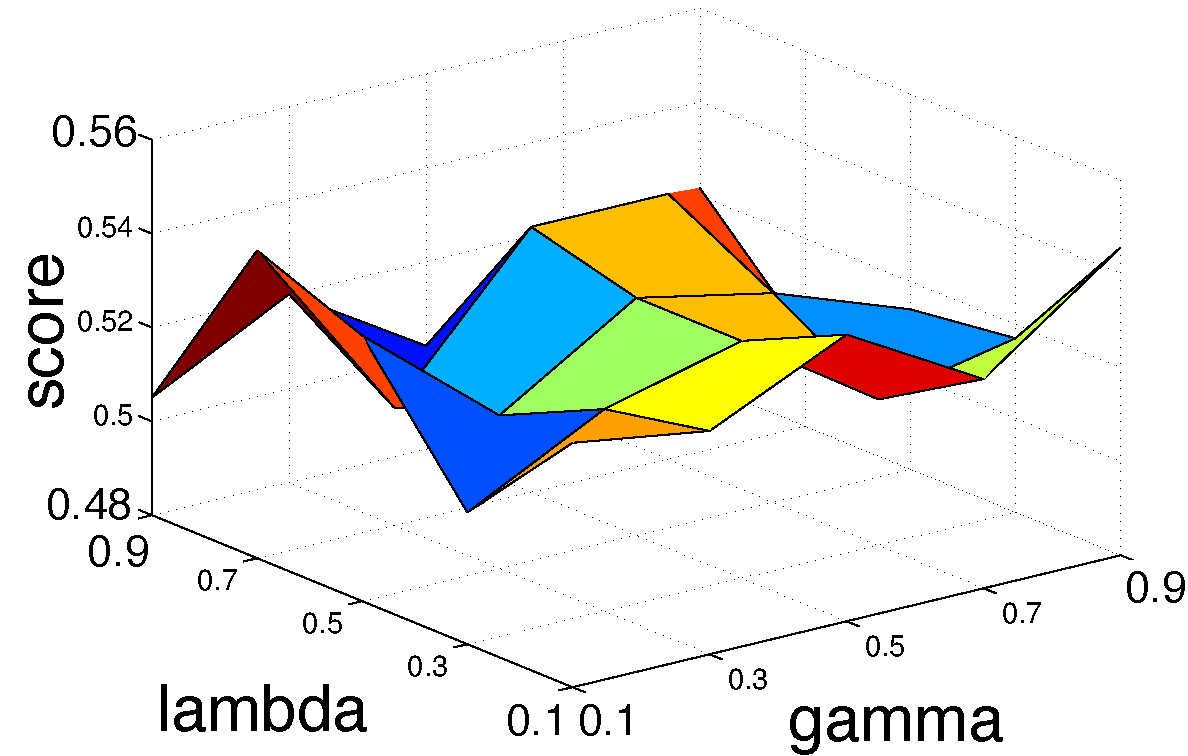
\includegraphics[width=0.5\linewidth]{img/alpha_analysis_30.pdf}}
%\includegraphics[width=0.5\linewidth]{img/wider_alpha_lambda.png}
\caption{Generalization score for the CCP trained with 0 obstacles with $\alpha = 0.1, 0.7$, the modal best alpha found during parameter analysis.
The remaining RL parameters $\gamma$ and $\lambda$ are shown on the X- and Y-axes. Bigger score is better. }
\label{fig:alpha_analysis_0obs}
\vspace{-5pt}
\end{figure}

\begin{figure}
\centering
\vspace{-5pt}
\subfloat[0 obstacles, $\gamma = 0.1$]{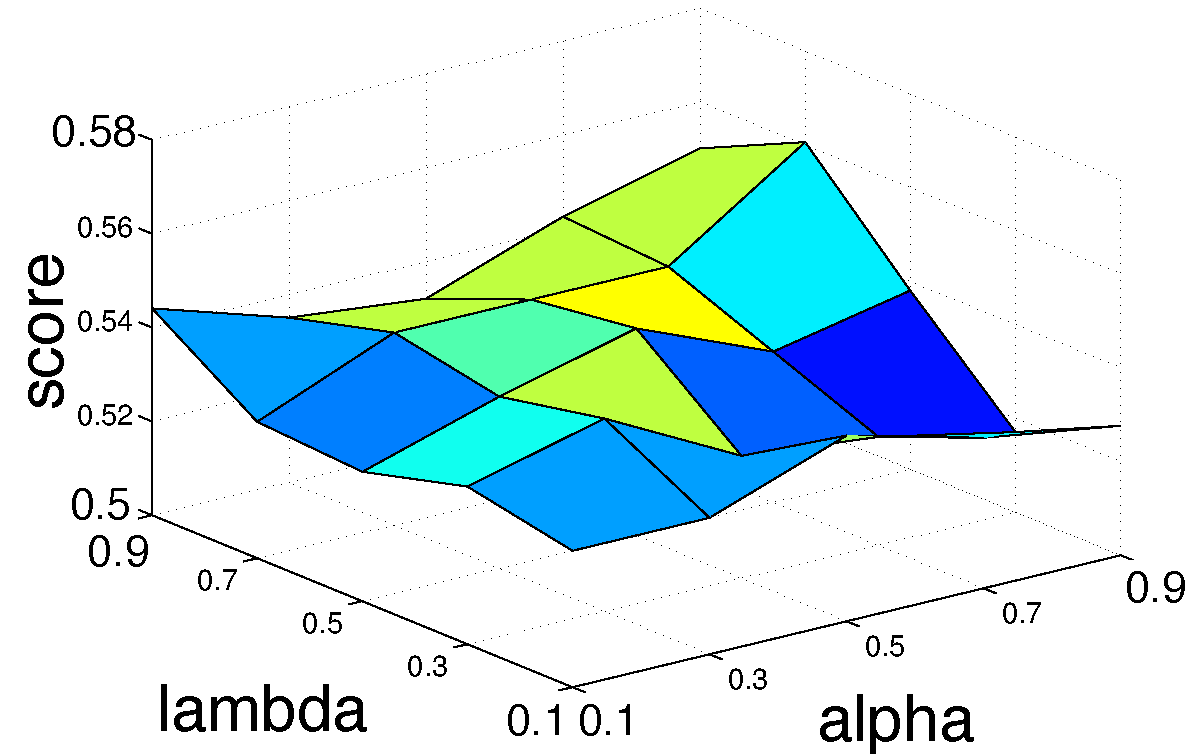
\includegraphics[width=0.5\linewidth]{img/gamma_analysis_0.pdf}}
\subfloat[30 obstacles, $\gamma = 0.3$]{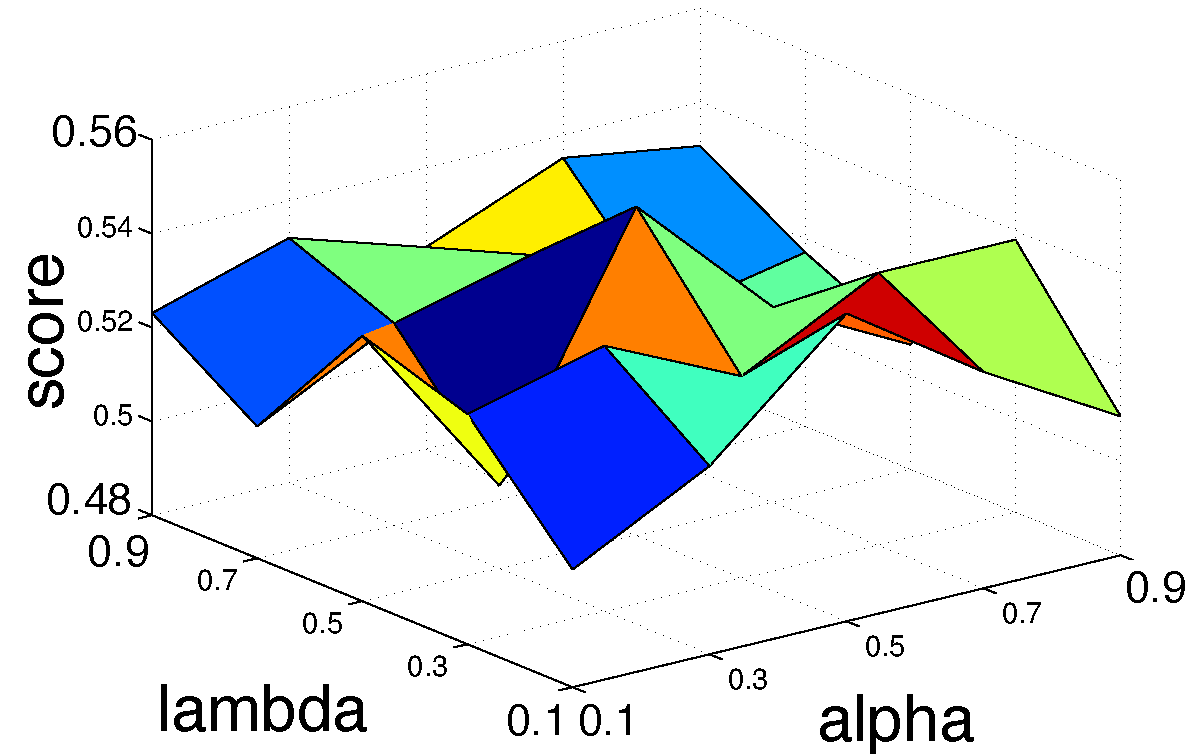
\includegraphics[width=0.5\linewidth]{img/gamma_analysis_30.pdf}}
%\includegraphics[width=0.5\linewidth]{img/wider_alpha_lambda.png}
\caption{Generalization score for the CCP trained with 0 obstacles with $\gamma = 0.1, 0.3$, the modal best gamma found during parameter analysis.
The remaining RL parameters $\alpha$ and $\lambda$ are shown on the X- and Y-axes. Bigger score is better. }
\label{fig:gamma_analysis_0obs}
\vspace{-5pt}
\end{figure}

\begin{figure}
\centering
\vspace{-5pt}
\subfloat[0 obstacles, $\lambda = 0.7$]{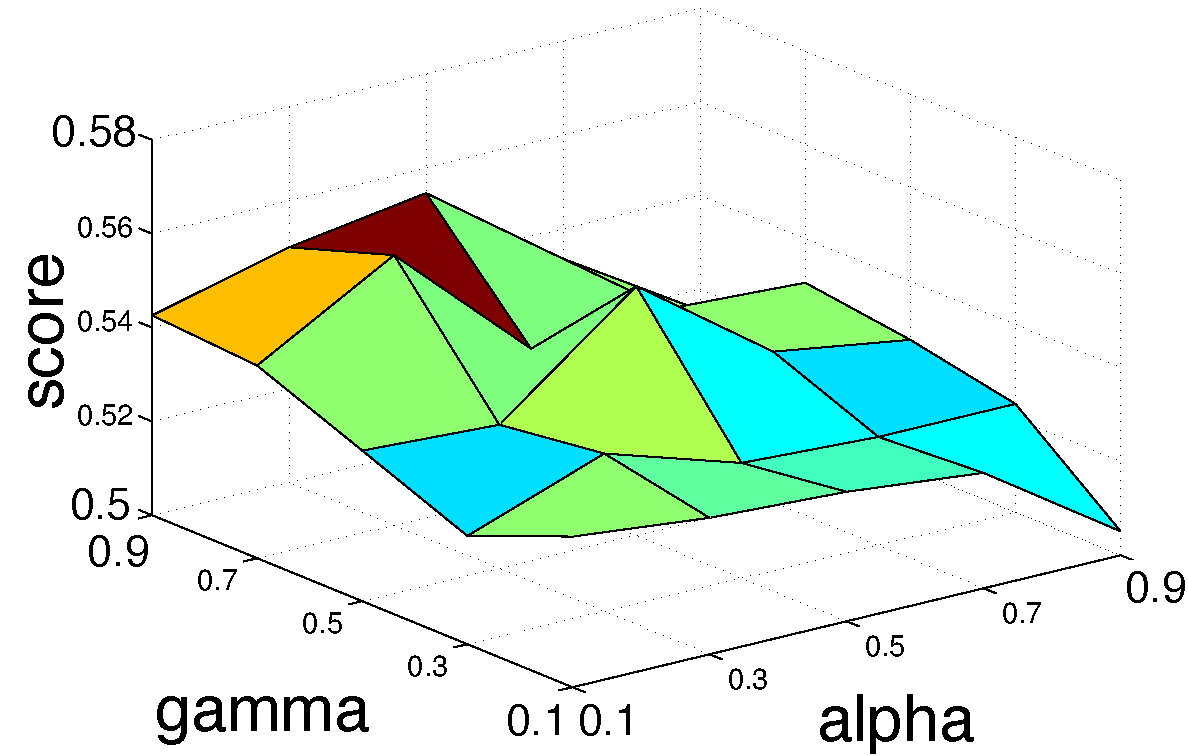
\includegraphics[width=0.5\linewidth]{img/lambda_analysis_0.pdf}}
\subfloat[30 obstacles, $\lambda = 0.5$]{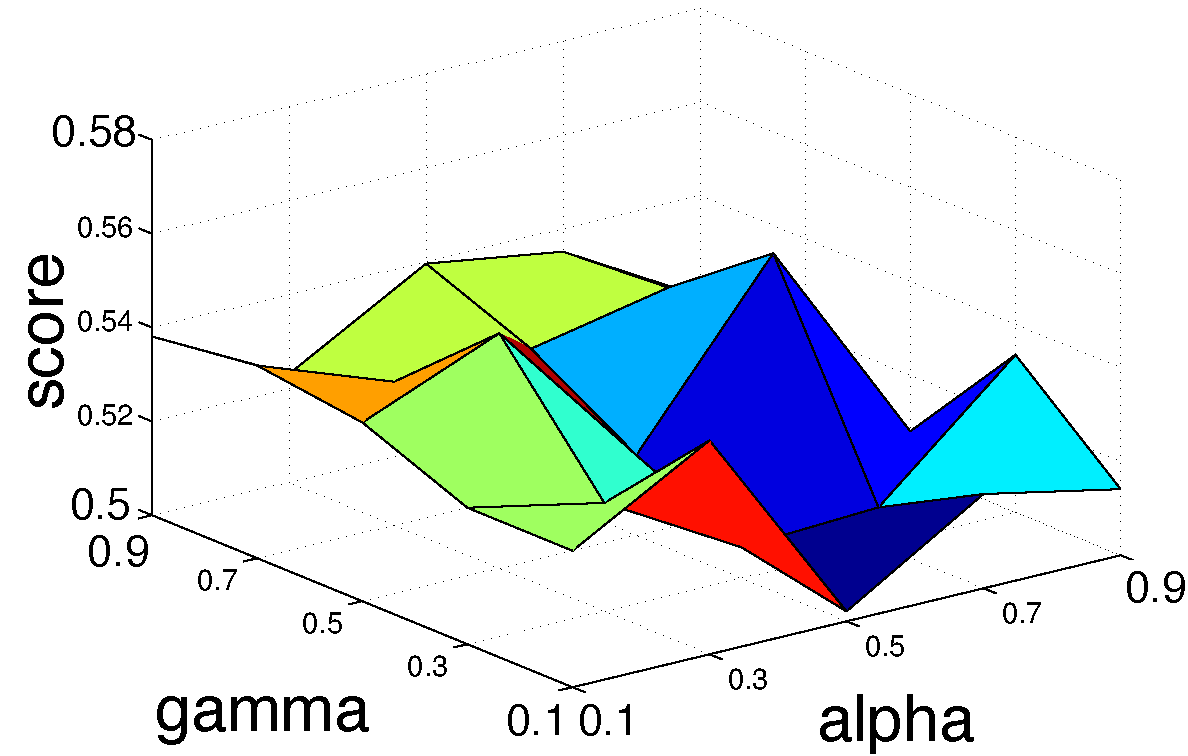
\includegraphics[width=0.5\linewidth]{img/lambda_analysis_30.pdf}}
%\includegraphics[width=0.5\linewidth]{img/wider_alpha_lambda.png}
\caption{Generalization score for the CCP trained with 0, 30 obstacles with $\lambda = 0.7, 0.5$, the modal best lambda found during parameter analysis.
The remaining RL parameters $\alpha$ and $\gamma$ are shown on the X- and Y-axes. Bigger score is better. }
\label{fig:lambda_analysis_0obs}
\vspace{-5pt}
\end{figure}

The learning rate, $\alpha$, controls how much the agent learns from the
error of its Q-function relative to the observed reward. Large values of
$\alpha$ can bias the agent towards behavioral feedback loops, by placing
emphasis on rewards experienced early in training. The parameter maps for
fixed values of $\alpha$ are shown in Figure \ref{fig:alpha_analysis_0obs}.
With a fixed value of alpha we see that there can be a wide range in behavior
as we vary the values of $\gamma$ and $\lambda$. The parametric performance
surface suggests that there may be multiple optima with these fixed $\alpha$
values for both the 0 and 30 obstacles cases. We will return to this observation
after examining the remaining parameters.

The discounting factor $\gamma$ encodes the discounting factor of future
rewards such that a reward 5 timesteps in the future is discounted by
a factor of $\gamma^{4}$. Agents with low values of $\gamma$ are relatively
short sighted, favoring actions that return larger immediate rewards at the
cost of longer-term considerations. The parameter maps for fixed values of
$\gamma$ are shown in Figure \ref{fig:gamma_analysis_0obs}. As we keep the
values of $\gamma$ fixed we see that for 0 obstacles large values of $\alpha$
and $\lambda$ lead to the best agent behavior. On the other hand, in the case
of 30 obstacles the best values of $\alpha$ and $\lambda$ are unclear, with
most pairings performing equivalently.  


\begin{table*}
\centering
\begin{tabular}{|r|r|r|r|}
\hline
\# Obstacles & Type & $score_{training}$ & $score_{test}$ \\
\hline
0 & RL & 0.99006(stdev 0.0022557) & 0.50496(stdev 0.0041289) \\
0 & GRN & 0.9945(stdev 0.0020109) & 0.52914(stdev 0.010029) \\
30 & RL & 0.43441(stdev 0.052902) & 0.49056(stdev 0.008722) \\
30 & GRN & 0.44452(stdev 0.047907) & 0.52326(stdev 0.014845) \\
\hline
\end{tabular}
\caption{Results for performance of RL with the best sampled parameters and
evolved GRN-controlled learning.
$score_{training}$ represents the fraction of dirt cleaned over all training
episodes (including initially naive behavior). $score_{test}$ represents the dirt that is
cleaned during a set of hypothetical scenarios. In both cases bigger is better.}
\label{tbl:result_comparison}
\end{table*}

\begin{figure}
\centering
\includegraphics[width=\linewidth]{img/best_per_seed_0.pdf}
\caption{Training (top) and generalization (bottom) scores for RL and neuromodulation per random seed for 0 obstacles.}
\label{fig:bestperseed0}
\vspace{-5pt}
\end{figure}

\begin{figure}
\centering
\includegraphics[width=\linewidth]{img/best_per_seed_30.pdf}
\caption{Training (top) and generalization (bottom) scores for RL and GRN per random seed for 30 obstacles.}
\label{fig:bestperseed30}
\vspace{-5pt}
\end{figure}

The trace decay $\lambda$ is used to discount the significance of actions
leading up to a reward. Larger values of $\lambda$ imply that the reward
an agent receives was highly dependent on a long sequence of actions that 
led to the reward. The parameter maps for fixed values of $\lambda$ are
shown in Figure \ref{fig:lambda_analysis_0obs}. Again, we see different
behavior for 0 and 30 obstacles. In the case of 0 obstacles it is fairly clear
that large values of $\gamma$ and small values of $\alpha$ are best. However,
in the case of 30 obstacle maps the performance of parameters is again noisier.
The highest peak is for $\alpha = 0.7$ and $\gamma = 0.5$. The non-uniformity
that is observed over the distribution of parameters leads us to consider that
the idea of choosing an optimal set of parameters is not only non-trivial, but
may not be possible. 


We see that parameter space can contain multiple optima and becomes more complex
as environmental complexity is increased. One might suspect that these multiple
optima correspond to different types of behavior that are learned by the RL agent.
Regardless of how the optima manifest in terms of behavior, the possibility of
dynamically adjusting the learning parameters to the RL agent may be a way of
harnessing the some of the properties of RL parameters over the course of a
series of training episodes. In the following section we present results for the 
dynamic control of the learning parameters by a GRN.

% Figure \ref{fig:alpha_lambda_generalization} shows the effect of $\alpha$ and
% $\lambda$ on the generalization of learned behavior.
% \begin{figure}
% \includegraphics[width=\linewidth]{img/wider_alpha_lambda.pdf}
% %\includegraphics[width=0.5\linewidth]{img/wider_alpha_lambda.png}
% \caption{Generalization score for a range of $\alpha$ learning rates and
% $\lambda$ trace decay rates. Bigger score is better. }
% \label{fig:alpha_lambda_generalization}
% \end{figure}

% It would be interesting if lambda was lower earlier, and higher later.

\section{Evolved Neuromodulation}

\begin{figure*}
\centering
\includegraphics[width=0.95\linewidth]{img/example_GRN_control_84.pdf}
\caption{Example of neuromodulation of learning and memory parameters $\alpha$, $\gamma$, and $\lambda$ by an evolved neuromodulatory GRN. 
This GRN is the best-of-run for a 30 obstacle map. These are the first 12
training episodes, where spikes at intervals of 200 indicate a resetting of the
environment.}
\vspace{-5pt}
\label{fig:exampleGRN}
\end{figure*}

In these experiments we present a comparison of the performance of uniformly
sampled RL parameters with the performance of GRN-controlled neuromodulation of
the same RL parameters. The dynamic control of learning and memory parameters by
this neuromodulatory process provides the agent with the means for adaptive
control of its own learning process. We show that agents who have been trained
with neuromodulatory GRNs controlling their learning and memory parameters, 
outperform RL agents that have been trained with fixed parameters. 

In Table \ref{tbl:result_comparison}, we see a comparison of RL agents that have
been trained with the best fixed parameters found with uniform sampling, and RL
agents that have been trained with neuromodulatory GRNs. Best fixed parameters
are a tuple of $(\alpha,\gamma,\lambda)$ that produce the highest score at the end
of training. Performance is compared
on the training map, as well as on a set of hypothetical scenarios designed to
test generalization. In the experiments with 0 obstacles, neuromodulatory GRNs
outperform fixed parameters in both training and test scores. The CCP with 0
obstacles is a relatively easy problem that can be solved with simple patterns
such as row-by-row cleaning. The improved performance with neuromodulation suggests
that the evolved GRN is guiding the reinforcement learning algorithm in meaningful
ways in response to environmenal cues. This is particularly visible in Figure
\ref{fig:bestperseed0} where neuromodulation is always better than pure
RL during training and for most tests. 

In experiments with 30 obstacles the results are not as clear-cut as in the case
of 0 obstacles. Figure \ref{fig:bestperseed30} details these result per
environment seed. Although the mean and standard deviation of training score for
neuromodulatory GRNs is slightly lower than those of fixed parameter RL, it is
not significant with respect to the standard deviation. However, agents trained
with neuromodulatory GRNs perform better on the set of hypothetical test scenarios.
This suggests that GRNs are not only guiding the RL algorithm in meaningful ways,
but that the GRN is helping the RL agent to learn generalizable behaviors. 

An example of one of the best-of-run GRNs from a 30 obstacle map is shown in
Figure \ref{fig:exampleGRN}. This figure shows an example training session with
a neuromodulatory GRN. While fixed parameter RL experiments maintain constant values
for $\alpha$, $\gamma$, and $\lambda$, the neuromodulatory GRN dynamically modulates
these learning and memory parameters. This particular GRN uses a strategy of a
high $\gamma$ value at the beginning of each training episode, which decays over the
course of the episode. $\lambda$ values are maintained near unity, which will 
heavily reinforce actions that have indirectly contributed to receiving a reward. Of
particular interest is the increase of $\alpha$ in response to decreases in $\gamma$.
This dynamic will cause agents to initially populate their Q-function relatively
quickly, and then will lead them to learn from their immediate rewards. This 
behavior can be particularly significant after most of the dirt has been removed
from the environment. Systematic errors which repeatedly leave dirt in similar
situations, such as those hard to reach corners that continually accumulate dust,
can be learned by these agents which begin to learn more from immediate rewards.

%SCB: both paragraphs are discussion => discussion & conclusion

\section{Discussion and Conclusions}

In this study we have introduced the evolution of neuromodulatory GRNs into the
framework of reinforcement learning by modulating both learning and memory
during on-line learning. Evolved neuromodulatory GRNs train RL agents that
consistently have improved generalization abilities relative to RL agents
trained with fixed parameter sets on the coverage control problem. The GRNs
dynamically adjust learning parameters relative to environmental inputs,
this dynamic adjustment allows agents to regulate changes in the behavior
by altering how behaviors are learned.

% SCB: both paragraphs :)
The Baldwin effect is a process in which learning allows an individual to
probe possible strategies. Successful strategies can then be evolved and incorporated into the genome by
selective pressures. However, this study approaches the Baldwin effect from
a different perspective than those of Hinton and Nowlan where
learning and evolution act on the same substrate, such as the weights of a 
neural network. In our case an evolved neuromodulatory GRN purely controls the learning
process. This is distinct from the Hinton and Nowlan class of experiments where learning,
in a sense, preceeds evolution which eventually learns fixed encodings of information
that would otherwise be learned. 

RL agents that are trained with neuromodulatory GRNs can outperform fixed parameter
RL agents in training environments in some cases; however, these GRNs consistently
train agents that have improved generalization capabilities. In this sense, the
neuromodulatory GRN serves as an excellent teacher to the RL agent, by guiding
the learning process in response to environmental variation. This may allow 
neuromodulated RL agents to utilize multiple phases of learning, whereby 
it is possible to learn how to correct previous mistakes. These reasons suggest
that it may be interesting to consider neuromodulatory GRNs within dynamic
environments, where learning on-the-fly can be critical.

Future work should investigate the effect of neuromodulatory GRNs in dynamic
environments, as well as in long-term evolution experiments. Extensions to
include additional neuromodulators, like those of \cite{Doya2002}, may further
improve performance. The enhanced generalization abilities of agents trained
with neuromodulatory GRNs suggests that this framework may be
useful in highly complex environments. Therefore, testing neuromodulatory GRNs
in other foraging tasks, such as hunting with high-dimensional visual input
\cite{Palmer2012}, may prove fruitful. Ultimately, neuromodulatory GRNs should
be studied in neural substrates of higher-order complexity.

\section{Acknowledgements}

We thank Yasmin Escobedo Lozoya, Jessica Lowell, Hava Siegelmann, and Richard
Watson for discussions that contributed to this work. We also thank Francesco
Pontiggia and the Brandeis HPC for providing computational support. 

%Brian

%\bibliographystyle{IEEEtran}
\bibliographystyle{plain}
\bibliography{../dissertation/library}
%\bibliography{bibtex}

\end{document}
